\documentclass[10pt]{article}
\usepackage{icmlko}

\icmlmeta{IP 파운데이션 월드모델}{247}{판이 못 보는 자리바꿈}{부호화 규약 하나가 아이돌을 $+$0.131 움직이는데 판은 0.004 밖에 안 움직인다}

\begin{document}

\twocolumn[
\icmlheader

\begin{abstract}
노트 240과 246이 같은 병을 두 번 짚었다 --- 손 축 다섯은 전 도메인이 계수를
\textbf{공유}하는데, 도메인마다 그 축의 \emph{분포}가 딴판이다(모바일
\texttt{entry\_friction} 은 값이 둘, 게임은 네 개, 웹툰은 연속에 가깝다).
그러니 하나의 계수가 서로 다른 눈금을 동시에 섬긴다. 자연스러운 구조 처방은
\textbf{도메인 안 백분위}로 분포를 맞추는 것이다 --- 순서는 그대로 두고
(동점은 동점으로 남는다) 주변 분포만 아홉 도메인에서 같게 만든다.
\textbf{판은 안 움직인다}: 손 축 다섯만 맞추면 $-$0.0036($t{=}-0.60$),
열일곱 축 전부면 $-$0.0047($t{=}-0.79$). 노트 245의 규약대로 정할 수 없는
자리다. \textbf{그런데 도메인은 크게 움직인다.} 아이돌 $+$0.131 · 게임
$-$0.084 · 도서 $-$0.025 · 웹툰 $+$0.024. 무게를 실어 더하면 움직인 총량이
$\sum w|\Delta| = 0.022$ 인데 판이 본 것은 $|\sum w\Delta| = 0.004$ 다 ---
\textbf{다섯 배가 상쇄돼 사라진다.} 자료는 한 글자도 안 바뀌었고 바뀐 것은
\emph{부호화 규약}뿐이다. 자리바꿈이 라벨 없이 예측되는지도 봤다 --- 그
도메인 축 분포가 남과 얼마나 다른가로 재면 spearman $-$0.351(n$=$9)로
쓸 수 없다. \textbf{판 $\rho$ 는 이 결정에 대해 잘못된 자다.} 안쪽으로도
못 정하고(0.004 는 노트 244의 신뢰도 아래) 유보로도 못 정하며(엿보기),
판으로도 못 정한다(상쇄). 그래서 안 바꾼다 --- 다만 \textbf{바꿀 수 없어서가
아니라 잴 자가 없어서}라고 적어 둔다.
\end{abstract}
]

\section{공유 계수를 고치는 자연스러운 길}

노트 246이 남긴 첫 갈래는 ``공유 계수 --- 손 축 다섯이 다 이렇다. 구조를
바꿀 길이 있나''였다. 노트 241이 길 하나를 이미 막았다(도메인별 기울기는
넷에서 손해, \texttt{entry\_friction} 은 $-$0.0309). 남은 길은 반대쪽이다 ---
기울기를 나누는 대신 \textbf{입력을 맞춘다}.

문제의 형태가 그것을 가리킨다. 같은 이름의 축인데 도메인마다 분포가 딴판이다.

\begin{center}\small
\begin{tabular}{lr}
\hline
\texttt{entry\_friction} & 서로 다른 값 \\
\hline
모바일 & 2 \\
게임 & 4 \\
웹툰 & 연속에 가까움 \\
\hline
\end{tabular}
\end{center}

하나의 계수가 이 셋을 동시에 섬긴다. 도메인 안 백분위로 바꾸면 순서는 그대로
남고(동점은 동점으로 남으므로 노트 240이 말한 \emph{고원}도 보존된다) 주변
분포만 아홉에서 같아진다.

\section{판은 안 움직인다}

\begin{center}\small
\begin{tabular}{lrrr}
\hline
 & F21 & F18 & F23 짝 차 \\
\hline
손 축 다섯만 & 0.4310 & 0.4392 & $-$0.0036 ($t{=}-0.60$) \\
열일곱 축 전부 & 0.4310 & 0.4394 & $-$0.0047 ($t{=}-0.79$) \\
\hline
\end{tabular}
\end{center}

둘 다 노트 245가 그은 0.010 선 안쪽이고 $t$ 가 1 도 안 된다. 그 규약대로면
여기서 멈춰야 한다 --- \textbf{정할 수 없는 자리}다. 그런데 도메인별로
열어 보니 멈추면 안 될 이유가 나왔다.

\section{도메인은 크게 움직인다}

\begin{figure}[t]
\centering
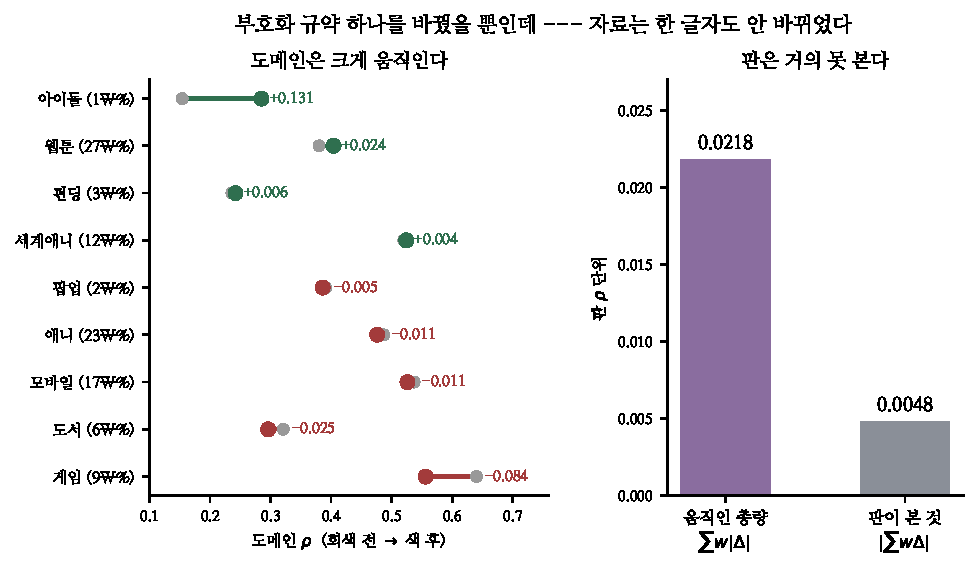
\includegraphics[width=\columnwidth]{figs/zerosum.pdf}
\caption{손 축 다섯을 도메인 안 백분위로 맞췄을 때. 자료는 안 바뀌었고
부호화 규약만 바뀌었다.}
\end{figure}

\begin{center}\small
\begin{tabular}{lrrrr}
\hline
도메인 & 몫 & 전 & 후 & 차 \\
\hline
아이돌 & 1.0\% & 0.154 & 0.285 & $\mathbf{+0.131}$ \\
웹툰 & 27.3\% & 0.380 & 0.404 & $+$0.024 \\
펀딩 & 3.1\% & 0.236 & 0.242 & $+$0.006 \\
세계애니 & 11.5\% & 0.520 & 0.524 & $+$0.004 \\
팝업 & 2.3\% & 0.391 & 0.386 & $-$0.005 \\
애니 & 23.2\% & 0.487 & 0.476 & $-$0.011 \\
모바일 & 16.9\% & 0.537 & 0.526 & $-$0.011 \\
도서 & 6.2\% & 0.321 & 0.296 & $-$0.025 \\
게임 & 8.6\% & 0.640 & 0.556 & $\mathbf{-0.084}$ \\
\hline
\end{tabular}
\end{center}

무게를 실어 더하면

\[ \sum_d w_d |\Delta_d| = 0.022, \qquad
   \Big| \sum_d w_d \Delta_d \Big| = 0.004. \]

\textbf{움직인 것의 다섯 중 넷이 상쇄돼 사라진다.} 판 $\rho$ 는 가중 평균이라
자리바꿈에 눈이 없다. 웹툰이 얻은 것을 게임이 내놓으면 판은 아무 일도 없었다고
보고한다.

\section{라벨 없이 예측되지 않는다}

자리바꿈이 미리 보이면 규약이 된다(노트 220 · 222 · 231 · 238 처럼). 제일
그럴듯한 짐작은 ``남과 분포가 많이 다른 도메인이 정규화로 제일 크게
움직인다''였다. 손 축마다 그 도메인 값과 나머지 전부의 값 사이 KS 거리를
평균해 견줬다.

\begin{center}\small
\begin{tabular}{lrr}
\hline
도메인 & 남과 다름 & 정규화 이득 \\
\hline
애니 & 0.605 & $-$0.011 \\
도서 & 0.509 & $-$0.025 \\
모바일 & 0.450 & $-$0.011 \\
아이돌 & 0.370 & $+$0.131 \\
게임 & 0.343 & $-$0.084 \\
웹툰 & 0.294 & $+$0.024 \\
\hline
\end{tabular}
\end{center}

spearman $-$0.351(n$=$9)이다. 부호도 짐작과 반대고 크기도 쓸 수 없다.
아이돌과 게임은 남과 다름이 거의 같은데(0.370 · 0.343) 이득은 $+$0.131 과
$-$0.084 로 갈린다. 반증.

\section{잴 자가 없다}

정리하면 이 결정에는 쓸 수 있는 자가 하나도 없다.

\begin{center}\small
\begin{tabular}{ll}
\hline
자 & 왜 못 쓰나 \\
\hline
안쪽 & 0.004 는 신뢰도 0.34 아래(노트 244) \\
유보 판 & 상쇄돼 0.004 밖에 안 보인다 \\
유보 도메인별 & 보이지만 그걸로 고르면 엿보기 \\
라벨 없는 짐작 & spearman $-$0.35, n$=$9 \\
\hline
\end{tabular}
\end{center}

그래서 안 바꾼다. 다만 \textbf{바꿀 이유가 없어서가 아니라 잴 자가 없어서}
안 바꾸는 것이고, 그 둘은 다르다. 노트 245는 ``작은 자리는 다투지 말라''고
했는데 이 노트가 단서를 붙인다 --- \textbf{판이 작다고 해서 변화가 작은
것은 아니다.} 판이 작은 이유가 상쇄일 수 있고, 그때 개별 도메인은 0.13 씩
움직이고 있다.

제품 쪽으로 곧장 붙는 함의가 있다. 도구가 파는 것은 판 $\rho$ 가 아니라
\textbf{한 도메인의 예측}이다. 아이돌만 쓰는 고객에게는 이 규약 하나가
$\rho$ 0.154 대 0.285 이고, 그건 우리가 지금껏 다툰 어떤 축보다 크다.

\paragraph{남은 것}
\begin{center}\small
\begin{tabular}{ll}
\hline
갈래 & 왜 \\
\hline
상쇄 진단 & $\sum w|\Delta|$ 를 판과 나란히 적으면 되나 \\
아이돌 & 25건인데 규약에 0.131 흔들린다. 왜 그렇게 약한가 \\
게임 & 정규화로 제일 많이 잃는다. 원 눈금이 게임에 맞춰져 있나 \\
도메인별 판정 & 판 하나로 고르는 것을 언제 그만두나 \\
\hline
\end{tabular}
\end{center}

\paragraph{규약} 판 짝 차가 0.010 안쪽이면 \textbf{$\sum w|\Delta|$ 를 같이
잰다.} 그것이 판보다 세 배 넘게 크면 ``효과 없음''이 아니라 \textbf{상쇄}이고,
상쇄는 보고해야 한다 --- 판정은 여전히 못 하더라도.

\end{document}
